\cleardoublepage
\chapter{The ROBOCEK Family}
\section{Vision}
\justify
    To devise a passionate community of strong responsible engineers technically skilled enough to figure out the need of the hour and act wisely to crack the challenges emphasizing the universal values.
\begin{marginfigure}
    
\includegraphics[width=\textwidth]{Images/ROBOCEK/ROBBOCEK_logo_black.png}
\end{marginfigure}

\section{Mission}
    To foster young minds into the ever evolving realm of robotics fabricating an ample learning environment aiding in design, operation and robotics with the aid of hands-on projects and collaborations with the experienced. 
\section{Values}
    Strives to excel as a learning community by adapting, learning and relentlessly improving ourselves and the entire team by promoting initiatives devising healthy, ethical and social relations adhering to sustainable models of development. 

\section{Down the Memory Lane}
\justify
A vibrant team of young enthusiasts from Govt. College of Engineering Kannur inspired from a group of students from Chennai, fabricated a small team with one dream to excel in the field of robotics. They named it \textit{\textbf{'Robotic Enthusiasts Of GCEK'}}. They hanged on to their dream of a robotics club for GCEK till it attained its official recognition on $30^{th}$ January, 2014.

\begin{figure}
    \centering
    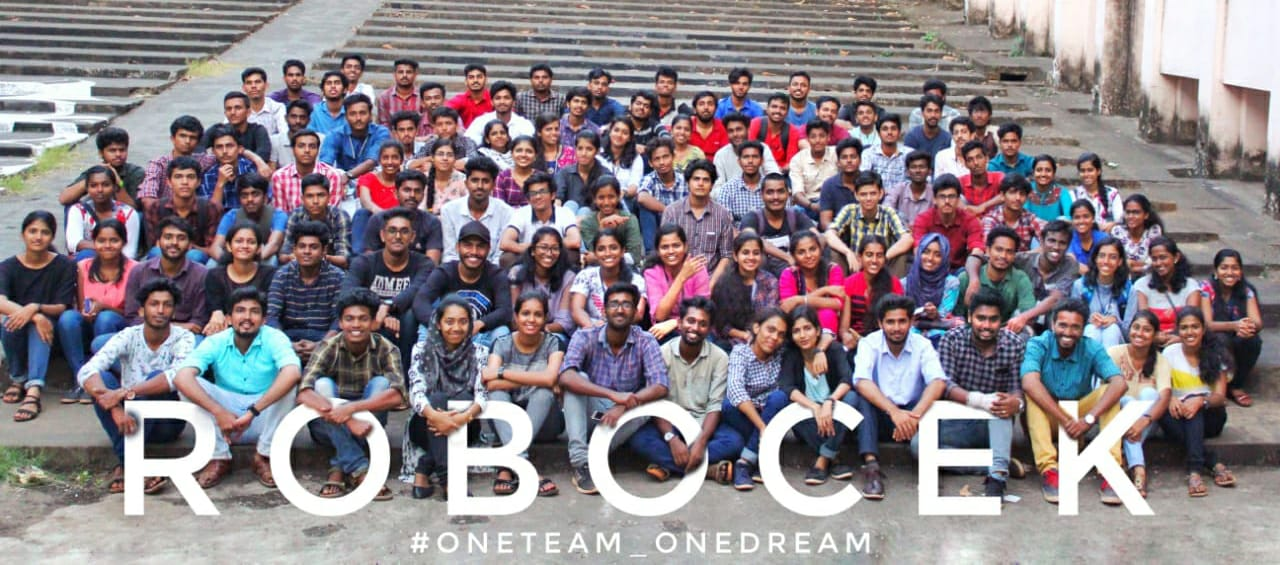
\includegraphics{Images/ROBOCEK/robocek.jpeg}
\end{figure}

\par ROBOCEK gradually evolved from a handful of members with no background in robotics into one of the most highly acclaimed robotics club in Kerala with a dedicated team and unmatched performance. The hardcore activities were accomplished by the students who organised themselves into an Executive Committee with prominent guidance from the Staff Advisors. They realised the dream of a room dedicated to ROBOCEK in GCEK. They conceived the idea of a basic workshop that would pave a path into the realm of robotics under ROBOCEK and finally converged to \textit{'ACTUATOR',The Beginner's Workshop}. Bit by bit 'Actuator' turned to be the first and the most interesting workshop that waved among the freshers of GCEK and also any entry point into the ROBOCEK. The pioneers into the club slowly engaged themselves into learning in groups.

The dedicated cluster of students strived to explore the intangible sphere of robotics through workshops, competitions, collaborative learning and expeditions nurturing academic excellence striving to keep in pace with electronics and robotics. The team endeavoured various tech fests, including national level fest - Xplore'19 and social relevant projects like expo's,flood relief activities, workshops etc.

\section{ROBOCEK Execom}
    \begin{figure*}
        \centering
        \subfloat{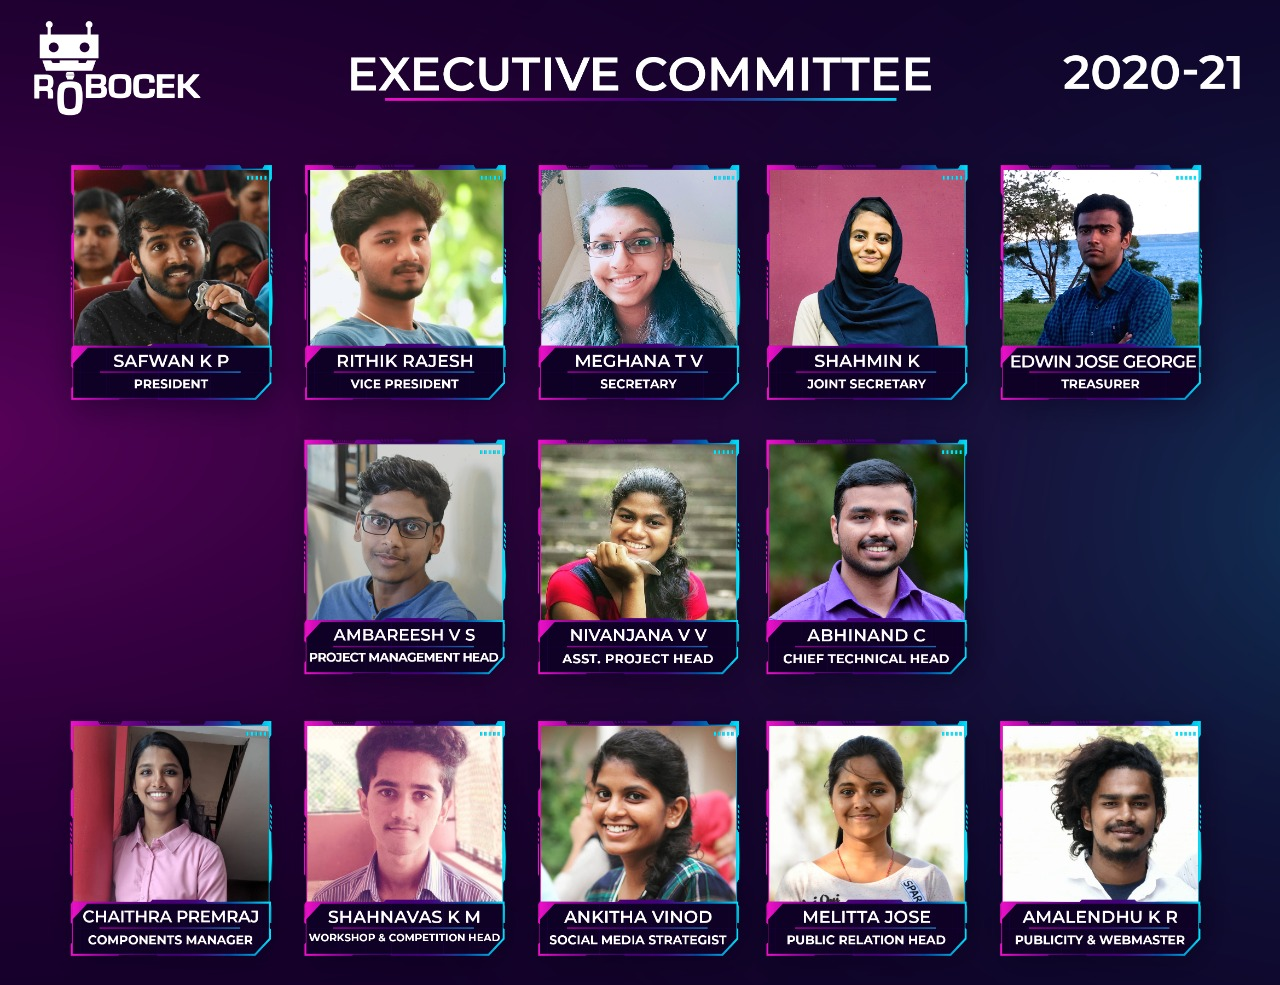
\includegraphics[width=2.7in]{Images/ROBOCEK/execom_2020_21.png}}\quad
        \subfloat{\includegraphics[width=2.7in]{Images/ROBOCEK/Advisory_Committee_2020_21_FinalDraft.png}}
    \end{figure*}
    
    \begin{figure*}
        \centering
        %\subfloat{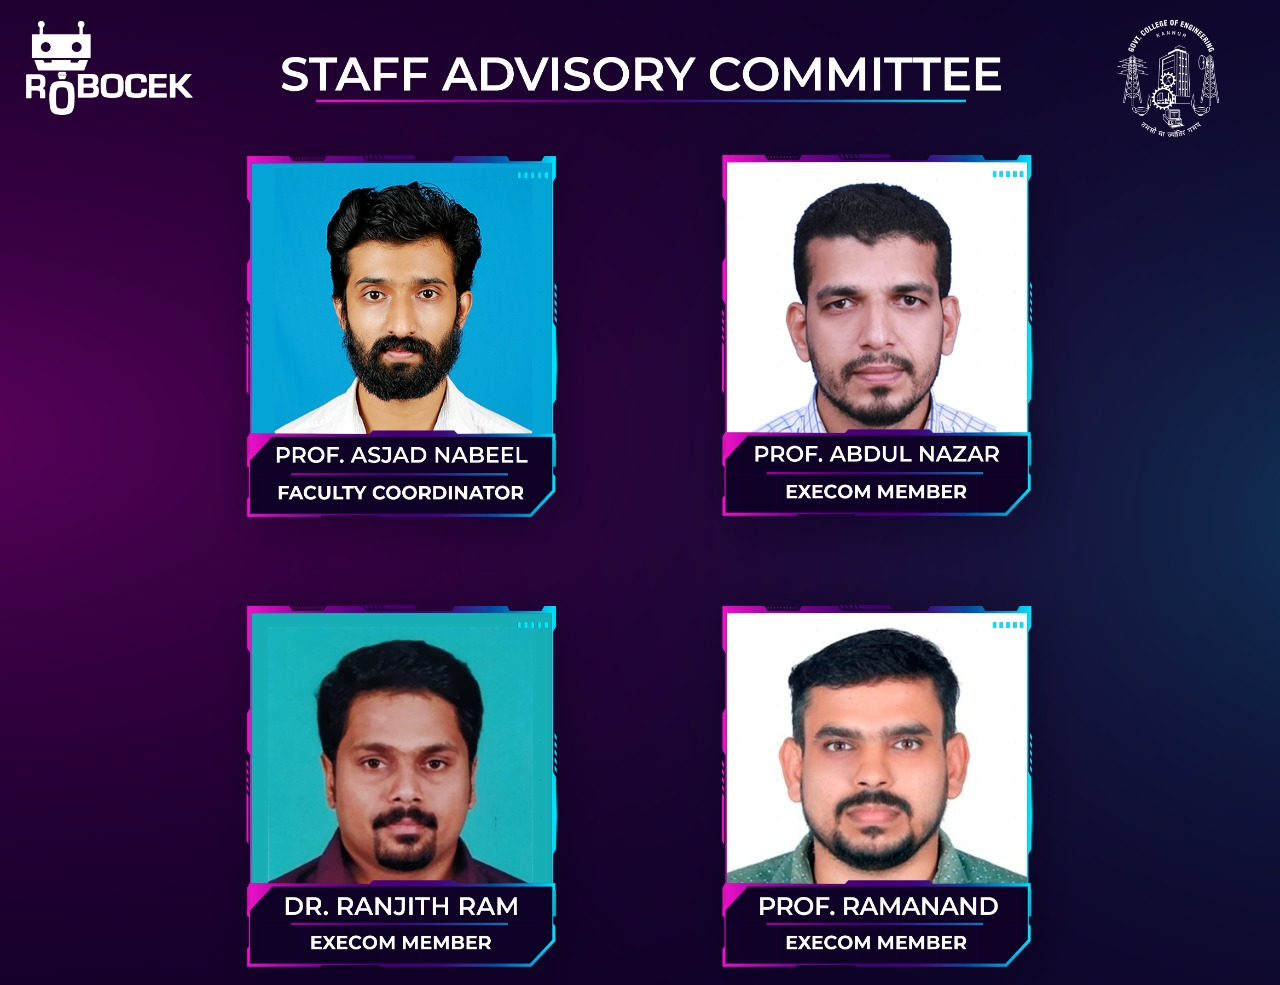
\includegraphics[width=2.7in]{Images/ROBOCEK/staff_advisors.jpeg}} \\
        \subfloat{\includegraphics[width=2.7in]{Images/ROBOCEK/execom_2019_20.jpg}}\quad
        \subfloat{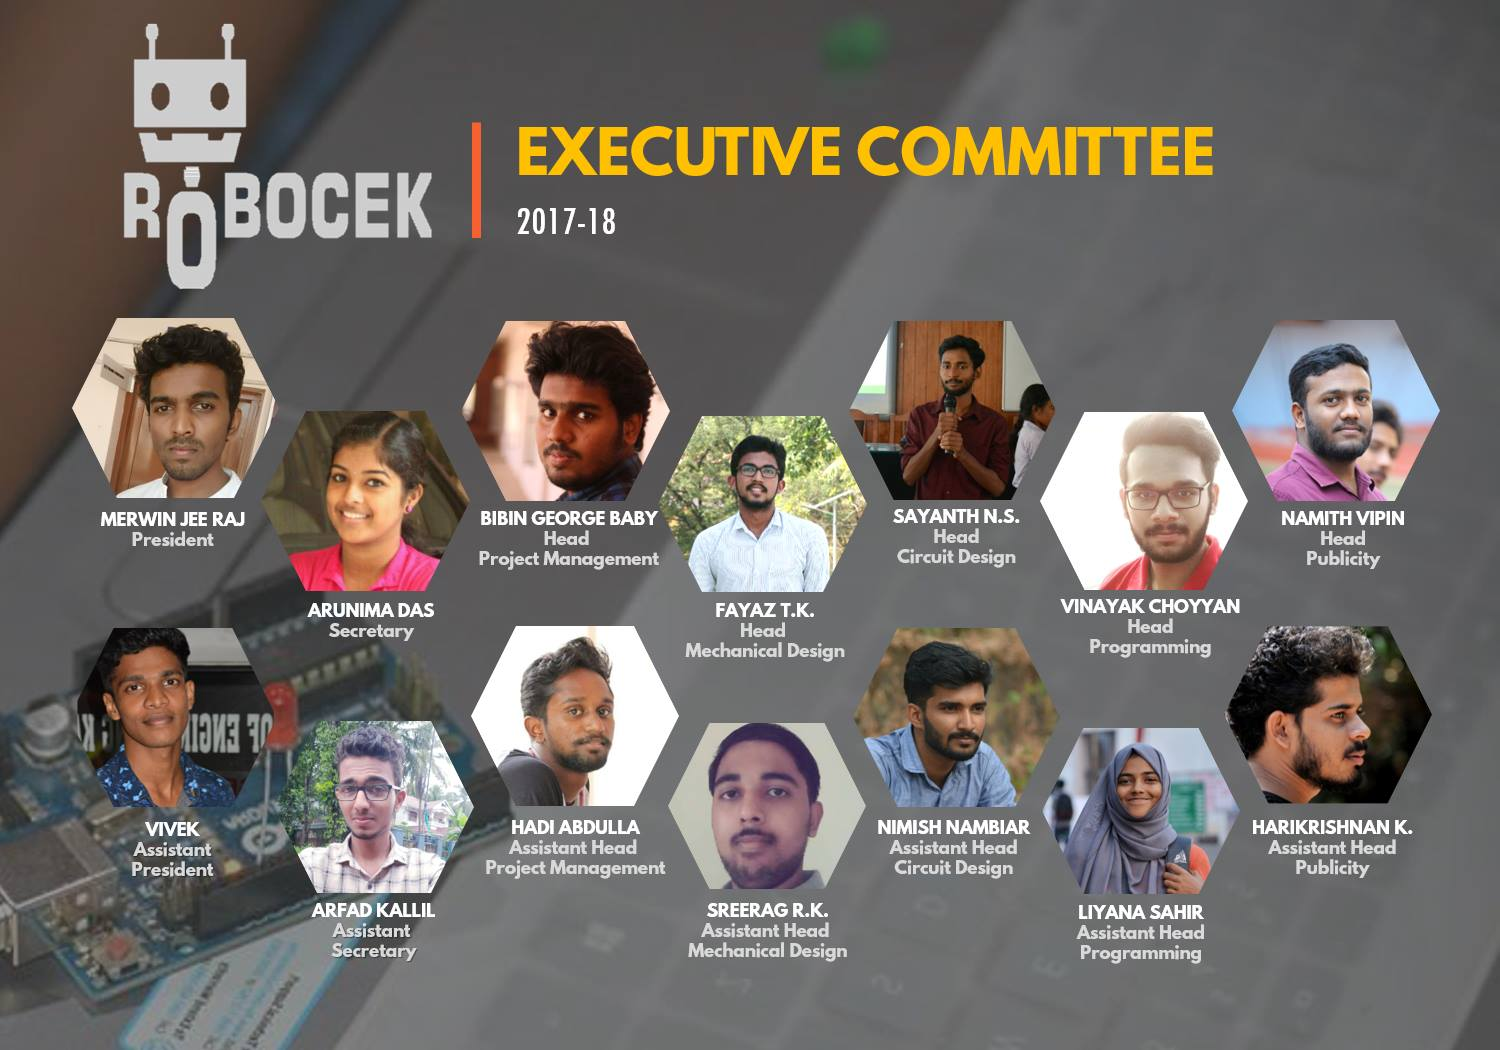
\includegraphics[width=2.7in]{Images/ROBOCEK/execom_2017_18.jpg}}
    \end{figure*}
    
    Its always been a proud moment to see an enthusiastic team that shape the progress of our club. Starting from 2014, <name> layed the foundation for the robotics club for the first time in GCE Kannur. Lead by <name>, striving through initial and difficult times, along with support from faculty, we payed a better way for the future generation of the college to invest their interest and passion in technology. With rising demand for betterment, an excellent team of enthusiastic students were chosen to drive ROBOCEK, meeting the vision and mission of the club. Though lead by a team, each and every innovations are always welcomed, helping the students to advance their career. Our courage to advance is the everlasting support from ROBOCEK Alumni, providing with examples and support for aspirants.

\newpage
\section{Reach out to us}
\begin{table}
\centering
    \begin{tabular}{ll}
    \ci{\faIcon{globe}}    & \url{https://robocek.org/}                            \\
    \ci{\faIcon{envelope}}  & \href{mailto: robocek@gcek.ac.in}{robocek@gcek.ac.in} \\
    \ci{\faIcon{envelope}}  & \href{mailto: robocek@gmail.com}{robocek@gmail.com} \\
    \ci{\faIcon{github}}    & \url{https://github.com/robocek} \\
    \ci{\faIcon{linkedin}}  & \url{https://www.linkedin.com/company/robocek/}       \\
    \ci{\faIcon{facebook}}  & \url{https://www.facebook.com/robocek/}               \\
    \ci{\faIcon{instagram}} & \url{https://www.instagram.com/robocek\_official/}      \\
    \ci{\faIcon{youtube}}   & \url{https://www.youtube.com/ROBOCEK}
    \end{tabular}
\end{table} 